\subsection{After fitting models with \texttt{lme4}}
\label{sec:afterfittingmodelswithlme4}

\paragraph{Basics and varying intercepts}

The output for GLMMs in \texttt{lme4} can be understood straightforwardly after what was said in Section~\ref{sec:fundamentals}.
Here is a possible output of the \texttt{summary} function for a fit of model (\ref{eq:glmm01}) and (\ref{eq:glmm02}), repeated as (\ref{eq:glmm01r}) and (\ref{eq:glmm02r}).
Artificial data were used.

\begin{align}
  P(y^i=1) & = logit^{-1}(\alpha_{l}^{j[i]}+\beta_d\cdot x_d^i)
  \label{eq:glmm01r} \\
  \alpha_l^j & \sim N(\mu_l,\sigma_l^2)
  \label{eq:glmm02r}
\end{align}

\vspace{0.5\baselineskip}

\begin{lstlisting}
Generalized linear mixed model fit by maximum likelihood 
 Family: binomial  ( logit )
Formula: construction ~ given + (1 | lemma)
   Data: observations
Random effects:
 Groups Name        Variance Std.Dev.
 lemma  (Intercept) 1.29     1.136   
Number of obs: 250, groups:  lemma, 5

Fixed effects:
            Estimate Std. Error z value Pr(>|z|)    
(Intercept)   0.7638     0.5513   1.385    0.166    
given1        1.5064     0.3626   4.154 3.26e-05 ***
\end{lstlisting}

Some clutter as well as information which we do not interpret here (AIC, BIC, and information about the residuals) have been removed.
In this output, the \texttt{(Intercept)} estimate ($0.7638$) is $\hat{\mu}_l$, and the \texttt{Variance} estimate for the \texttt{lemma} random intercept ($1.29$) is $\hat{\sigma}_l^2$.%
\footnote{The notation $\hat{v}$ is used to denote and estimate of or a prediction for the variable $v$.}
The estimate for \texttt{given1} ($1.5064$) corresponds to $\hat{\beta}_d$.
Finally, we learn that there were five different lemmas and $250$ observations in total.

To see whether the random intercept has a considerable influence, we should first look at the variance estimate.
Here, it is larger than $1$, which would be surprising if there were nothing going on in terms of between-lemma variation.
It is possible to compute confidence intervals for the variance estimate using the \texttt{confint} function.
Assuming the original model was stored in \texttt{alternation}, the following two alternatives work.

\vspace{0.5\baselineskip}

\begin{lstlisting}
  confint(alternation, parm="theta_", method = "profile")
  confint(alternation, parm="theta_", method = "boot",
          nsim = 250)
\end{lstlisting}

The profile method uses LR tests and the bootstrap method uses a parametric bootstrap.
For this model (where the variance estimate was $1.29$ and the true value used to generate the data was $1.5$), the profile method gives $0.5808\dots2.6433$ and the bootstrap with $250$ simulations gives $3.9665\cdot10^{-6}\dots1.8023$ as the $95\%$ confidence interval.
Since the bootstrap (especially with smaller original sample sizes as in this case) typically tends to run into replications where the estimation of the variance fails and is thus returned as $0$, the bootstrap interval is skewed to the left, while the profile confidence interval frames the true value symmetrically.
The bootstrap is thus not always more robust or intrinsically better.

Although the authors of the \texttt{lme4} package advise against it, a significance test on the deviances of a simple GLM and a GLMM with an added single random effect can be performed with the \texttt{anova} function.

\vspace{0.5\baselineskip}

\begin{lstlisting}
alternation.0 <- glm(construction ~ given,
                     data = observations,
		     family = binomial(link=logit))
anova(alternation, alternation.0)
\end{lstlisting}

The GLMM object must be the first argument to \texttt{anova}.
In this case, the output looks like this, indicating a significant effect, although the p-values should not be considered highly reliable.

\vspace{0.5\baselineskip}

\begin{lstlisting}
Data: observations
Models:
alternation.0: construction ~ given
alternation:   construction ~ given + (1 | lemma)
             Df  logLik deviance  Chisq Df Pr(>Chisq)    
alternation.0 2 -134.52   269.05                         
alternation   3 -119.12   238.24 30.801  1  2.859e-08 ***
\end{lstlisting}

If the nested (simpler) model still contains a random effect, the \texttt{update} function can be used to build the simpler model.
Also, in addition to the \texttt{anova} command, there is a drop-in replacement for LR tests using bootstrap methods in the \texttt{pbkrtest} package \citep{HalekohHojsgaard2014}.

\vspace{0.5\baselineskip}

\begin{lstlisting}
alternation.1 <- glmer(construction ~ given +
                       (1 | lemma) + (1 | semantics),
	               family = binominal(link=logit),
		       data = my.data)
alternation.2 <- update(object = alternation,
                        formula = construction ~
			          given +
                                  (1 + | lemma))

require(pbkrtest)
PBmodcomp(alternation.1, alternation.2, nsim = 250)
\end{lstlisting}

The coefficient of determination (pseudo-$R^2$) according to \citet{NakagawaSchielzeth2013} can be computed using the function \texttt{r.squaredGLMM} from the \texttt{MuMIn} package \citep{Barton2016}.

\vspace{0.5\baselineskip}

\begin{lstlisting}
require(MuMIn)
r.squaredGLMM(alternation)
\end{lstlisting}

In this case, it gives us \texttt{R2m = 0.1101} and \texttt{R2c = 0.3608}, so there is a considerable difference between the marginal $R^2$ (without random effects) and conditional $R^2$ (with random effects).

To inspect the conditional modes, the \texttt{ranef} function can be used, and it can also output standard errors for them.

\vspace{0.5\baselineskip}

\begin{lstlisting}
ranef(alternation, drop = T, condVar = T)
\end{lstlisting}

% To plot the predictions for the levels of a random effect, packages like \texttt{sjPlot} offer customisable functions, as in the following example, which plots Figure~\ref{fig:blups}.
% Notice that calls the conditional modes BLUPs (best linear unbiased predictors), which is an alternative term for conditional means in linear models.
% 
% \vspace{0.5\baselineskip}
% 
% \begin{lstlisting}
% sjp.glmer(alternation, sort.est = "sort.all",
%           facet.grid = F, show.ci = T)
% \end{lstlisting}
% 
% \begin{figure}[!htpb]
%   \centering
%   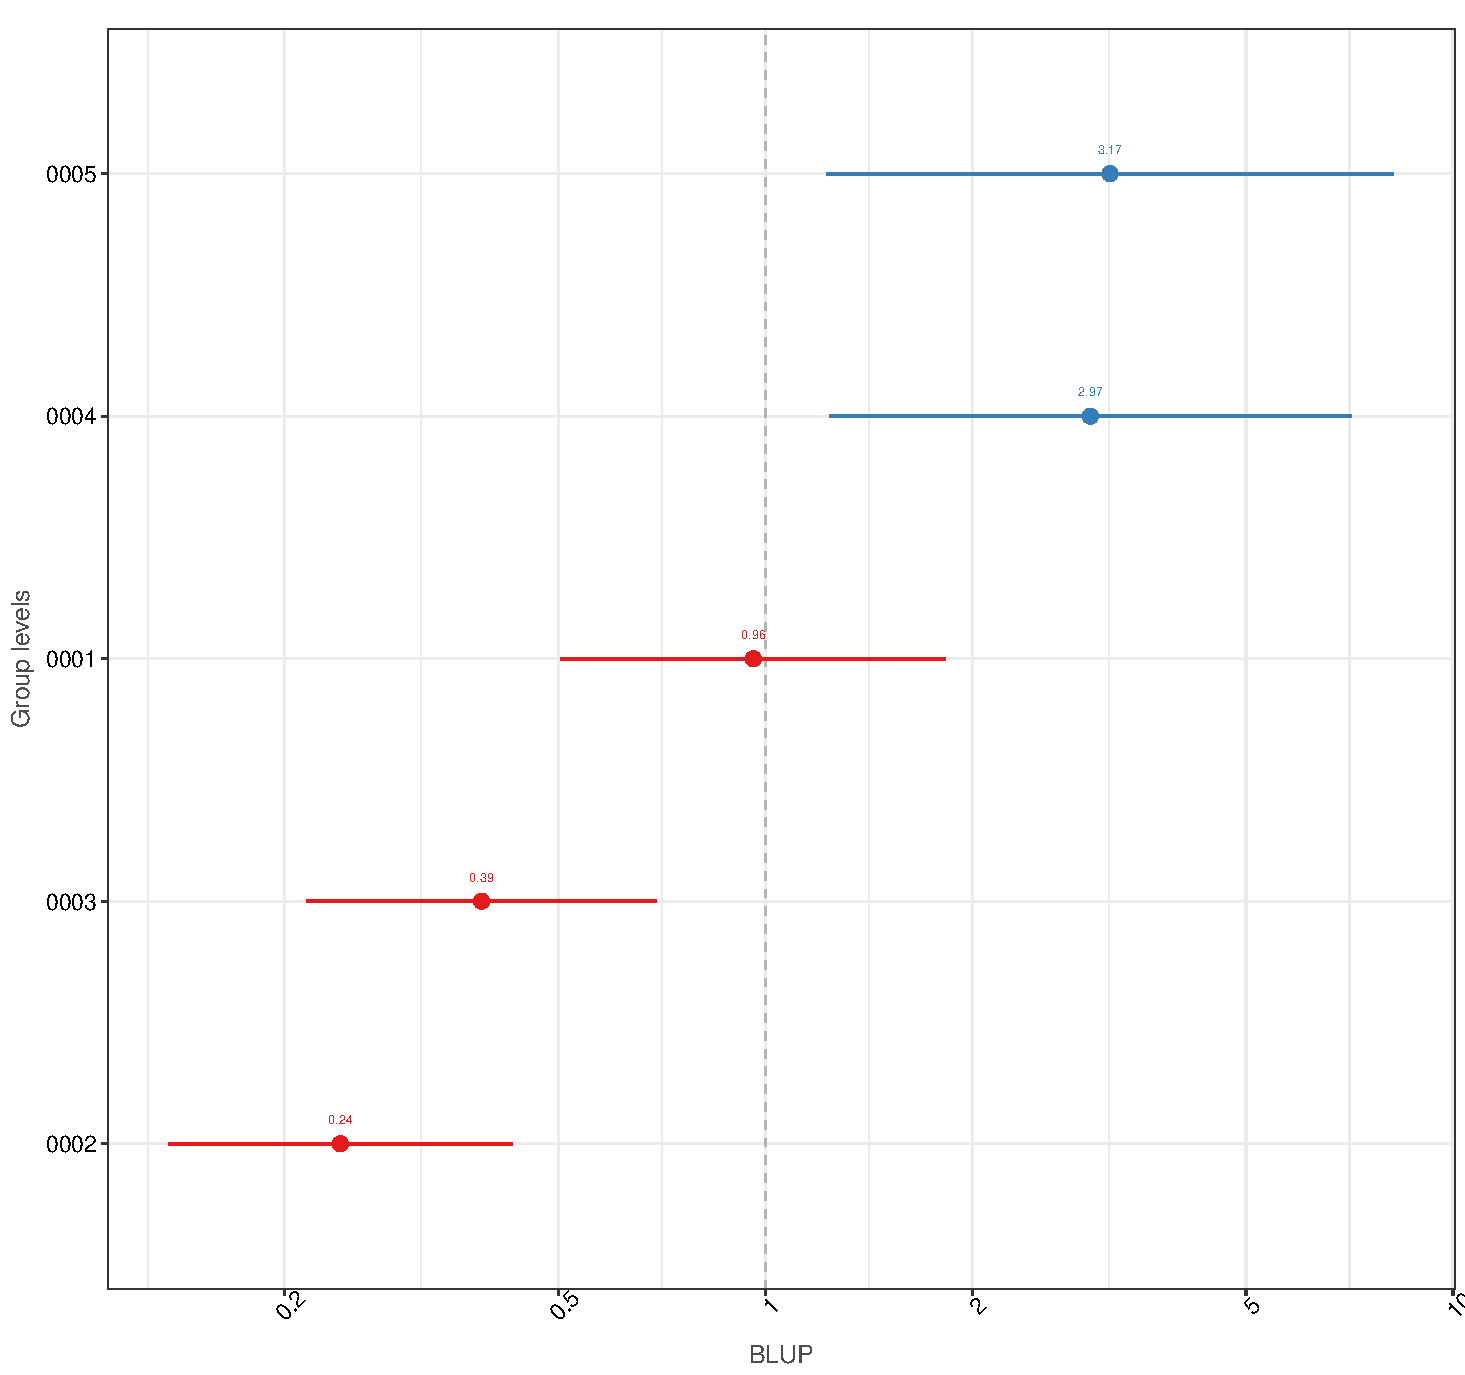
\includegraphics[width=0.9\textwidth]{graphics/blups}
%   \caption{Estimated conditional modes with prediction intervals}
%   \label{fig:blups}
% \end{figure}

\paragraph{Varying intercepts and slopes}

In the \texttt{summary} output for a VIVS model such as (\ref{eq:glmm05}), the columns \texttt{Variance} and \texttt{Corr} can be regarded as specifying the lower triangle of the variance-covariance matrix.%
\footnote{Alternatively, the \texttt{VarCorr} function could be used to extract this information.}

\vspace{0.5\baselineskip}

\begin{lstlisting}
Random effects:
 Groups Name        Variance Std.Dev. Corr 
 lemma  (Intercept) 0.6103   0.7812        
        given       0.8944   0.9457   -0.39
Number of obs: 2500, groups:  lemma, 50

Fixed effects:
            Estimate Std. Error z value Pr(>|z|)    
(Intercept)   0.6332     0.1226   5.163 2.43e-07 ***
given        -1.0428     0.1492  -6.990 2.75e-12 ***
\end{lstlisting}

This output tells us that the estimated variance in the intercepts is $\hat{\sigma}_{\alpha}^2=0.6103$, the estimated variance in the slopes is $\hat{\sigma}_{\beta}^2=0.8944$, and the covariance coefficient estimate is $\hat{\rho}=-0.39$ (a healthy value inasmuch as it is not $1$ or $-1$).
The means are estimated as $\hat{\mu}_{\alpha}=0.6332$ and $\hat{\mu}_{\beta}=-1.0428$.
Compare this to Section~\ref{sec:morecomplexmodels}, especially (\ref{eq:glmm06}).
It is possible to reconstruct group-wise models from this output and a lookup of the group-specific predictions using the \texttt{ranef} function.
For the first group, for example, the following can be done.

\vspace{0.5\baselineskip}

\begin{lstlisting}
ranef(alternation)$lemma[1,]
\end{lstlisting}

The output is as follows.

\vspace{0.5\baselineskip}

\begin{lstlisting}
     (Intercept) given
0001   0.4351156 -1.227842
\end{lstlisting}

This means that for the first lemma, actual predictions for the outcome of the alternation can be made using (\ref{eq:glmm012}), where values are rounded to two decimal digits.
Compare this to (\ref{eq:glmm05}).

\begin{equation}
  Pr(y^i=1)=logit^{-1}( [0.63+0.44] + [-1.04-1.23]\cdot x_d^i )
  \label{eq:glmm012}
\end{equation}

% \subsection{Summary and recommendations for a protocol}
% \label{sec:summaryandrecommendationsforaprotocol}
% 
% In this chapter, readers should have learned that the output of \texttt{R} is transparent when practitioners are able to relate it to (1) the structure of their data set and (2) the specification of the model.
% As a general protocol, it is recommended that for each study, researchers first examine their data set, then specify a model in mathematical notation \textit{including the variance-covariance matrix} based on their knowledge of the data and the theory behind their study.
% After the re-specification in \texttt{R} and the estimation, the \texttt{R} output and the model specification can be easily related, and informed inferences can be made.

